\documentclass[a4paper]{scrartcl}

%\usepackage{showframe}
\usepackage[margin=2cm,footskip=.7cm]{geometry}
\usepackage{enumitem}
% \usepackage{fourier}
\usepackage{xcolor}
% \usepackage{abkuerzungen}
\usepackage{hyperref}
\usepackage{amsmath}
\usepackage{../../ISASmacros/isasmathmacros}

\usepackage{pdfpages}


\newcommand{\sA}{\ensuremath{\mathsf{A}}}
\newcommand{\sAB}{\ensuremath{\mathsf{AB}}}
\newcommand{\sB}{\ensuremath{\mathsf{B}}}
\newcommand{\sBA}{\ensuremath{\mathsf{BA}}}
\newcommand{\sC}{\ensuremath{\mathsf{C}}}

\newcommand{\cest}{\ensuremath{\cvec{\gamma}}}
\newcommand{\cerest}{\ensuremath{\ervec{\gamma}}}
\newcommand{\cmat}{\ensuremath{\mat{\Gamma}}}
\newcommand{\tmat}{\ensuremath{\widetilde{\mat{\Gamma}}}}

\newcommand{\gainA}{\ensuremath{\mat{K}}}
\newcommand{\gainB}{\ensuremath{\mat{L}}}

% \newcommand{\fus}{\ensuremath{\op{fus}}}

% \newcommand{\CI}{\op{CI}\xspace}
% \newcommand{\EI}{\op{EI}\xspace}
% \newcommand{\ICI}{\op{ICI}\xspace}
% \newcommand{\BC}{\op{B\!/\!C}\xspace}
% \newcommand{\ind}{\op{s}\xspace}
\newcommand{\ind}{\op{in}\xspace}
\newcommand{\opt}{\cmat}


\newcommand{\excmat}{\ensuremath{\mat{\Gamma}'}}
\newcommand{\excest}{\ensuremath{\cest'}}
% \newcommand{\exoptmat}{\ensuremath{\mat{C}_{\excmat}}}
\newcommand{\exoptmat}{\ensuremath{\mat{C}'_\EI}}

%\RequirePackage[mathscr]{euscript}
%\RequirePackage{bbding}
%\RequirePackage{scalefnt}
%\RequirePackage{mathtools}
% This was enabled but makes the text look ugly
%\RequirePackage[T1]{fontenc}


%%% COLOR DEFINITIONS

% KIT Colors
\definecolor{kitgreenex}{RGB}{0,152,131}
\definecolor{kitblueex}{RGB}{52,115,186}
\definecolor{kitmaygreen}{RGB}{119,184,38}
\definecolor{kityellow}{RGB}{255,228,0}
\definecolor{kitorange}{RGB}{247,154,0}
\definecolor{kitbrown}{RGB}{182,130,28}
\definecolor{kitred}{RGB}{187,25,23}
\definecolor{kitpurple}{RGB}{190,0,126}
\definecolor{kitcyanblue}{RGB}{0,167,227}
% Own Definitions
\definecolor{grey}{RGB}{150,150,150}


\definecolor{nblue}{RGB}{54,95,145}

%%% FONTS
%\setkomafont{pageheadfoot}{\small\color{darkgray}}
%\setkomafont{pagefoot}{\normalfont\color{darkgray}}
%\setkomafont{pagenumber}{\color{darkgray}}
%\setkomafont{captionlabel}{\small\bfseries\color{darkgray}}
\setkomafont{disposition}{\bfseries}
\setkomafont{section}{\normalfont\large\bfseries}
\setkomafont{subsection}{\normalfont\bfseries}
\setkomafont{author}{\normalfont}
\setkomafont{date}{\normalfont}


%%% PARAGRAPH LAYOUT
\setlength{\parindent}{0mm}
\setlength{\parskip}{6pt}


%%% REBUTTAL COMMANDS
\newenvironment{rebuttal}{\begin{enumerate}[label={\color{grey}\thesection.\arabic{enumi}},leftmargin=0pt,ref=\thesection.\arabic{enumi}]}{\end{enumerate}}
\newcommand{\reviewtext}[1]{{\color{nblue} #1}}
\newcommand{\papertext}[1]{\emph{``#1''}}

%%% HYPERREF SETUP
\hypersetup{
        colorlinks = true,
        linkcolor = kitgreenex
}

%%%%%%%%%%%%%%%%%%%%%%%%%%%%%%%%%%%%%%%%%%%%%%%%%%%%%%%%%%%%%%%%%%%%%%%%

\title{\boldmath Distributed Range-Only Localisation that Preserves Sensor and Navigator Privacies}
\subtitle{Response to Reviewers' Comments - Submission IEEE-TAC 21-1548}
\author{Marko Ristic\and Benjamin Noack\and Uwe D. Hanebeck}

%       .d8888b.  888                     888
%      d88P  Y88b 888                     888
%      Y88b.      888                     888
%       "Y888b.   888888  8888b.  888d888 888888
%          "Y88b. 888        "88b 888P"   888
%            "888 888    .d888888 888     888
%      Y88b  d88P Y88b.  888  888 888     Y88b.
%       "Y8888P"   "Y888 "Y888888 888      "Y888

\begin{document}

\maketitle

Dear Prof. David Castanon,\\
Dear Reviewers,

Thank you all for the positive reviews, in this letter we will address the remaining comments and changes made to the manuscript. Throughout this response, reviewers' comments are in \reviewtext{blue}. 

Sincerely,\\
Marko Ristic, Benjamin Noack, and Uwe D. Hanebeck

%      8888888888     888 d8b 888
%      888            888 Y8P 888
%      888            888     888
%      8888888    .d88888 888 888888 .d88b.  888d888
%      888       d88" 888 888 888   d88""88b 888P"
%      888       888  888 888 888   888  888 888
%      888       Y88b 888 888 Y88b. Y88..88P 888
%      8888888888 "Y88888 888  "Y888 "Y88P"  888



\section*{Response to the Editor's Report}
\def\thesection{E}
\begin{rebuttal} %\setcounter{enumi}{-1}
\item \reviewtext{I am pleased to inform you that the paper is acceptable for publication in the Transactions provided that you can make the modifications described below.

The reviewers would like the authors to double check the symbols and formulas and clarify some concerns on sensor attacks etc, which are detailed in their comments.}

We are glad to hear the positive response, thank you. Below we clarify the remaining concerns from reviewer comments.

\end{rebuttal}

%      8888888b.                         d888
%      888   Y88b                       d8888
%      888    888                         888
%      888   d88P .d88b.  888  888        888
%      8888888P" d8P  Y8b 888  888        888
%      888 T88b  88888888 Y88  88P        888
%      888  T88b Y8b.      Y8bd8P         888
%      888   T88b "Y8888    Y88P        8888888



\section*{Response to the Comments of Reviewer 1 (262567)}
\def\thesection{R1}
\begin{rebuttal}
\item \reviewtext{Based on the revision, all my concerns have been addressed well now I recommend accepting this manuscript as it is.}

We are happy to hear this is the case, thank you.

\end{rebuttal}

%      8888888b.                         .d8888b.
%      888   Y88b                       d88P  Y88b
%      888    888                              888
%      888   d88P .d88b.  888  888           .d88P
%      8888888P" d8P  Y8b 888  888       .od888P"
%      888 T88b  88888888 Y88  88P      d88P"
%      888  T88b Y8b.      Y8bd8P       888"
%      888   T88b "Y8888    Y88P        888888888



\section*{Response to the Comments of Reviewer 2 (262571)}
\def\thesection{R2}
\begin{rebuttal}
\item \reviewtext{This paper presents a range-only localisation method meeting formal cryptographic requirements that ensure sensors keep their measurements, sensor variances and locations private while the navigator keeps its estimates private. The paper is standardized and the mathematical derivation seems correct, but there are still some areas that need to be improved, please check and correct.

1. In Notation, please correct the sentence ``$\|$ the binary concatination operator''.}

Thank you for the supportive comments. The quoted sentence has been updated.

\item \reviewtext{2. In section II-A, please check the correctness of the formula $l_i^{(t)}=\sum_{j=1}^m a^{(t)}_{j,i} \omega^{(t)}_i$, which is inconsistent with the description in Fig. 1.}

The error has now been corrected, thank you for noticing it.

\item \reviewtext{3. In section II-A, is the sensor Honest-but-Curious or is the attacker model Honest-but-Curious? How does the attack occur in the sensors?}

This was not written clearly and we are grateful that it was pointed out. The section has been updated to explicitly state that attackers are honest-but-curious and that the navigator or sensors can be corrupted. We hope this clarifies the intended meaning.

\item \reviewtext{4. What's the meaning of $\mathcal{E}(\cdot)$ in $\mathsf{CombEnc}(t,pk_0,sk_i,\mathcal{E}(\omega_1^{(t)}),\dots)$? The author does not give a paraphrase in Notation. And in $\mathsf{AggDec}(t,pk_0,sk_0,\dots)$, the public and private keys $pk_0,sk_0$ is not shown in the description of linear combinations $\sum_{i=1}^n l_i^{(t)} = \sum_{i=1}^n \sum_{j=1}^m a^{(t)}_{i,j} \omega^{(t)}_j$.}

The reviewer is correct to notice the inconsistency with notations in this section. Key subscripts have been added to make it clear that the encryptions $\mathcal{E}(\cdot)$ are performed with the keys generated in the $\mathsf{Setup}(\cdot)$ algorithm and the linear combinations $l_i^{(t)}$ modified to denote the unencrypted sum.

\item \reviewtext{5. Please complete the references with the relevant information, for example, the year of publication of ref. 8.}

Sorry about the mistake, the missing year has been added and the remaining references inspected for additional errors.

\end{rebuttal}

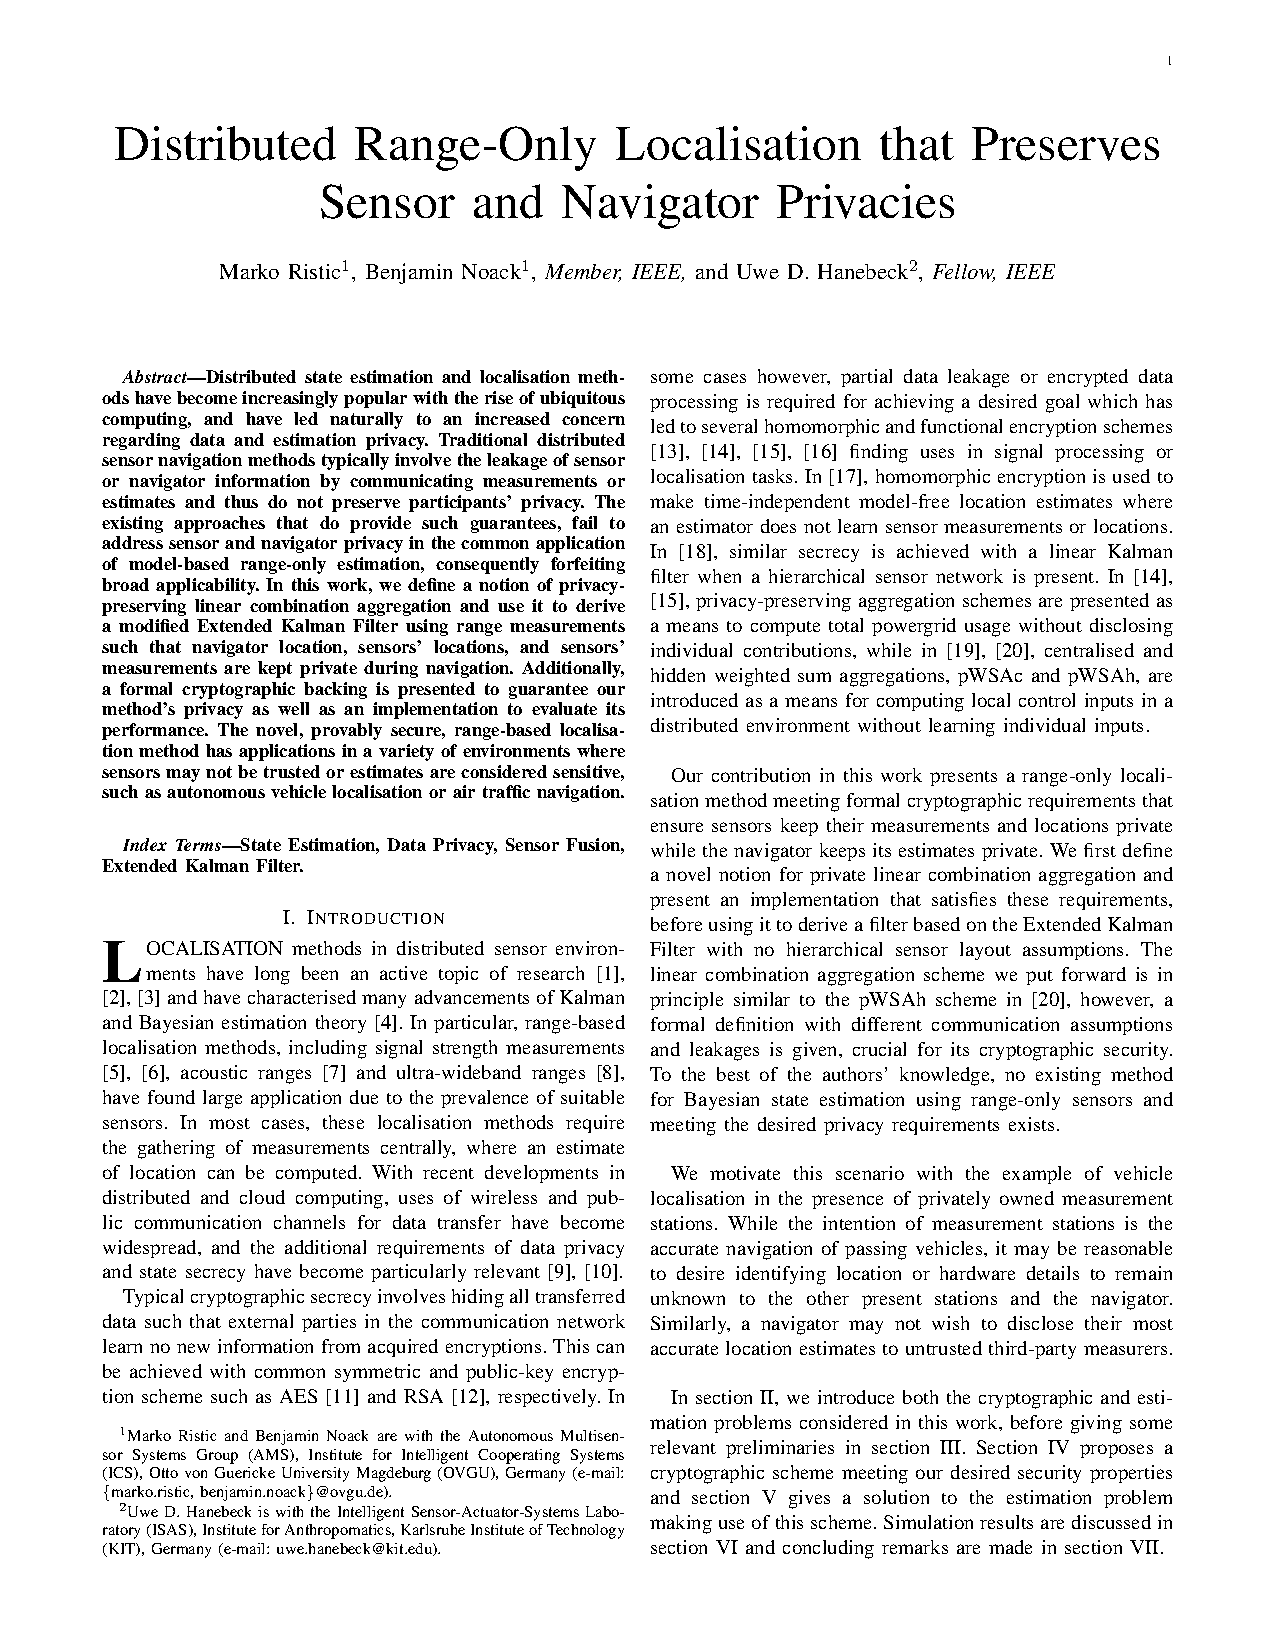
\includepdf[pages=-]{../../diff.pdf}

\end{document}